\documentclass[10pt]{standalone}
\usepackage{amsmath}
\usepackage{amssymb}
\usepackage{pgf,tikz}
\usepackage{mathrsfs}
\usetikzlibrary{arrows}
\pagestyle{empty}

\begin{document}

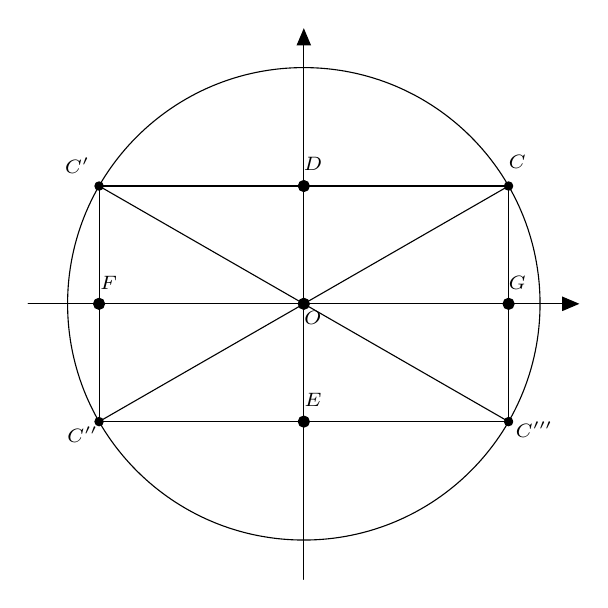
\begin{tikzpicture}[line cap=round,line join=round,>=triangle 45,x=1.0cm,y=1.0cm]

\draw[->] (-3.5,0.) -- (3.5,0.);

\draw[->] (0.,-3.5) -- (0.,3.5);


\clip(-3.5,-3.5) rectangle (3.5,3.5);

\draw  (0.,0.) circle (3.cm);
\draw  (-2.6004106645141394,1.495949322631329)-- (2.6004106645141394,1.4959493226313287);
\draw  (-2.6004106645141394,1.495949322631329)-- (-2.6004106645141394,-1.495949322631329);
\draw  (-2.6004106645141394,-1.495949322631329)-- (2.6004106645141394,-1.4959493226313292);
\draw  (2.6004106645141394,1.4959493226313287)-- (2.6004106645141394,-1.4959493226313292);
\draw  (0.,0.)-- (2.6004106645141394,1.4959493226313287);
\draw  (0.,0.)-- (-2.6004106645141394,1.495949322631329);
\draw  (0.,0.)-- (-2.6004106645141394,-1.495949322631329);
\draw  (0.,0.)-- (2.6004106645141394,-1.4959493226313292);
\begin{scriptsize}
\draw [fill=black] (0.,0.) circle (2.0pt);
\draw[color=black] (0.11550413223140407,-0.17694710743801595) node {$O$};

\draw [fill=black] (2.6004106645141394,1.4959493226313287) circle (1.5pt);
\draw[color=black] (2.710545454545455,1.806523966942149) node {$C$};
\draw [fill=black] (-2.6004106645141394,1.495949322631329) circle (1.5pt);
\draw[color=black] (-2.8762314049586797,1.756937190082645) node {$C'$};

\draw [fill=black] (-2.6004106645141394,-1.495949322631329) circle (1.5pt);
\draw[color=black] (-2.810115702479341,-1.6645504132231397) node {$C''$};
\draw [fill=black] (2.6004106645141394,-1.4959493226313292) circle (1.5pt);
\draw[color=black] (2.9254214876033062,-1.5984347107438008) node {$C'''$};
\draw [fill=black] (0.,1.495949322631329) circle (2.0pt);
\draw[color=black] (0.11550413223140407,1.7734661157024796) node {$D$};
\draw [fill=black] (0.,-1.495949322631329) circle (2.0pt);
\draw[color=black] (0.11550413223140407,-1.2182694214876024) node {$E$};
\draw [fill=black] (-2.6004106645141394,0.) circle (2.0pt);
\draw[color=black] (-2.479537190082647,0.26933388429752114) node {$F$};
\draw [fill=black] (2.6004106645141394,0.) circle (2.0pt);
\draw[color=black] (2.710545454545455,0.26933388429752114) node {$G$};
\end{scriptsize}
\end{tikzpicture}
\end{document}